% RAG deployment / service architecture (docker-compose stack)
% Compile: pdflatex rag_deployment.tex
% Transparent PNG: gs -sDEVICE=pngalpha -r300 -o rag_deployment.png rag_deployment.pdf
\documentclass[tikz,border=12pt]{standalone}
\usepackage{tikz}
\usetikzlibrary{positioning,arrows.meta,shapes.geometric,fit,backgrounds,calc}

\begin{document}
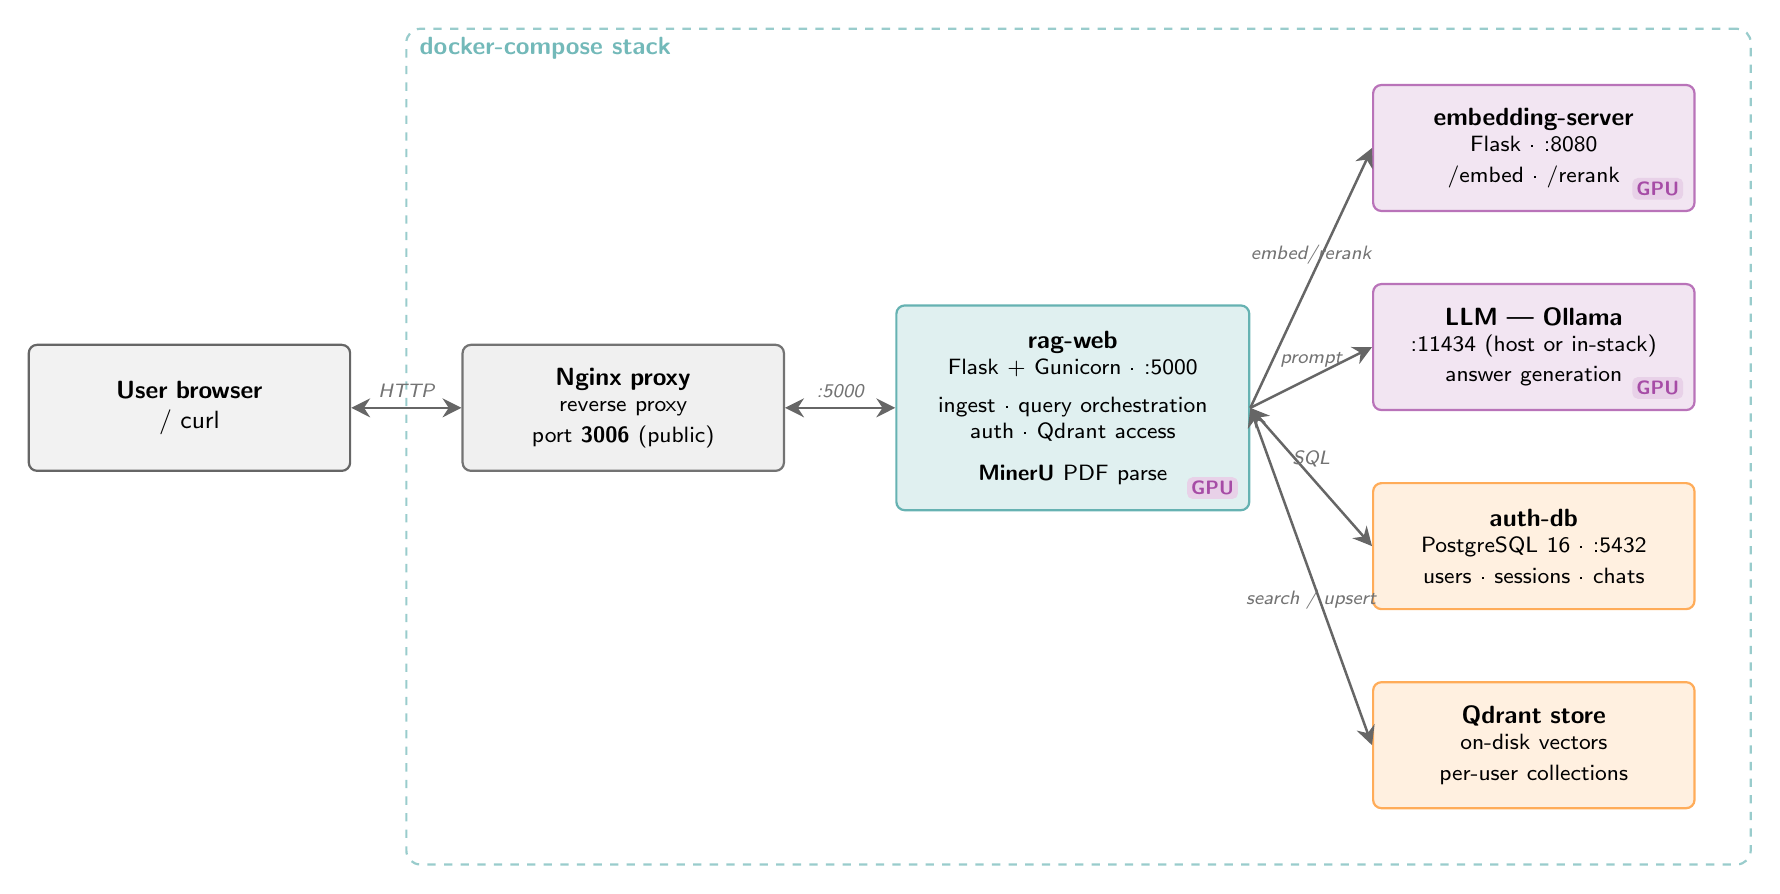
\begin{tikzpicture}[
    font=\sffamily,
    svc/.style={
        rounded corners=3pt, draw=black!55, line width=0.8pt,
        text width=38mm, minimum height=16mm, align=center,
        inner sep=4pt, font=\sffamily\small, fill=black!3},
    client/.style={svc, fill=black!5,   draw=black!60},
    edge/.style={svc,   fill=gray!12,    draw=black!55},
    web/.style={svc,    fill=teal!12,    draw=teal!60, text width=42mm, minimum height=26mm},
    gpu/.style={svc,    fill=violet!10,  draw=violet!55},
    data/.style={svc,   fill=orange!12,  draw=orange!65},
    link/.style={-{Stealth[length=2.4mm,width=2.4mm]}, line width=0.9pt, draw=black!60},
    bilink/.style={{Stealth[length=2.4mm,width=2.4mm]}-{Stealth[length=2.4mm,width=2.4mm]},
                   line width=0.9pt, draw=black!60},
    tag/.style={font=\scriptsize\sffamily\itshape, text=black!55},
    gtag/.style={font=\scriptsize\sffamily\bfseries, fill=violet!18,
                 text=violet!70, rounded corners=2pt, inner sep=1.5pt},
]

% ---- client + edge (left column) ----
\node[client] (user) {\textbf{User browser}\\ / curl};
\node[edge, right=14mm of user] (proxy) {\textbf{Nginx proxy}\\ \footnotesize reverse proxy\\ \footnotesize port \textbf{3006} (public)};

% ---- rag-web hub (centre) ----
\node[web, right=14mm of proxy] (web)
    {\textbf{rag-web}\\ \footnotesize Flask + Gunicorn · :5000\\[4pt]
     \footnotesize ingest · query orchestration\\ \footnotesize auth · Qdrant access\\[4pt]
     \footnotesize \textbf{MinerU} PDF parse};

% ---- backing services (right column, stacked) ----
\node[gpu]  (embed) at ($(web.east)+(36mm,33mm)$)
    {\textbf{embedding-server}\\ \footnotesize Flask · :8080\\ \footnotesize /embed · /rerank};
\node[gpu, below=9mm of embed]  (llm)
    {\textbf{LLM — Ollama}\\ \footnotesize :11434 (host or in-stack)\\ \footnotesize answer generation};
\node[data, below=9mm of llm]   (pg)
    {\textbf{auth-db}\\ \footnotesize PostgreSQL 16 · :5432\\ \footnotesize users · sessions · chats};
\node[data, below=9mm of pg]    (qdrant)
    {\textbf{Qdrant store}\\ \footnotesize on-disk vectors\\ \footnotesize per-user collections};

% ---- GPU corner badges ----
\node[gtag, anchor=south east, xshift=-1.5mm, yshift=1.5mm] at (web.south east)   {GPU};
\node[gtag, anchor=south east, xshift=-1.5mm, yshift=1.5mm] at (embed.south east) {GPU};
\node[gtag, anchor=south east, xshift=-1.5mm, yshift=1.5mm] at (llm.south east)   {GPU};

% ---- links ----
\draw[bilink] (user)  -- (proxy) node[midway,above,tag]{HTTP};
\draw[bilink] (proxy) -- (web)   node[midway,above,tag]{:5000};
\draw[link] (web.east) -- (embed.west)  node[midway,above,tag,yshift=1pt]{embed/rerank};
\draw[link] (web.east) -- (llm.west)    node[midway,above,tag]{prompt};
\draw[bilink] (web.east) -- (pg.west)   node[midway,above,tag]{SQL};
\draw[bilink] (web.east) -- (qdrant.west) node[midway,below,tag,yshift=-1pt]{search / upsert};

% ---- frame ----
\begin{scope}[on background layer]
    \node[draw=teal!40, line width=0.8pt, rounded corners=5pt, dashed,
          fit=(proxy)(web)(embed)(llm)(pg)(qdrant),
          inner sep=7mm, label={[anchor=north west,font=\sffamily\bfseries\small,
          text=teal!55]north west:\,docker-compose stack}] (box) {};
\end{scope}

\end{tikzpicture}
\end{document}
